\pagebreak
\chapter[Introduction]{}\vspace{-2cm}\noindent\rule{\textwidth}{2.5pt}
\thispagestyle{empty}

\vspace{5cm}\textbf{\huge{Introduction}}

\medskip\noindent\rule{\textwidth}{1pt}

As NASA prepares to return to the Moon, innumerable activities to equip, shelter, and otherwise support future astronauts are underway.  These astronauts will be eating and drinking, and subsequently urinating and defecating in microgravity and lunar gravity.  While astronauts are in the cabin and out of their spacesuits, they will need a toilet that has all the same capabilities as ones here on Earth. NASA is calling on the global community for their novel design concepts for compact toilets that can operate in both microgravity and lunar gravity.  These designs may be adapted for use in the Artemis lunar landers that take us back to the Moon.  Although space toilets already exist and are in use (at the International Space Station, for example), they are designed for microgravity only.  NASA’s Human Landing System Program is looking for a next-generation device that is smaller, more efficient, and capable of working in both microgravity and lunar gravity. This challenge includes a Technical category and Junior category.

\pagebreak
It is in this calling of this unique challenge that we wish to provide a solution that is both functional and innovative. This document will provide our design rationale, the functionality of the product, and how this design has innovated prior designs.  

\section[Space Waste Collection Systems]{Overview of Space Waste Collection Systems}
Space Waste Collection Systems(WCS) are the implementation of Earth toilets in a microgravity environment. However, easier said than done while in microgravity there poses a challenge of transporting and storing human waste. While in microgravity, fluids are pulled together through its surface tension causing the mundane task of transporting anything through a fluid system a non-trivial task. As a result of this non-trivial task, this seemingly simple task on Earth becomes a very intensive engineering project that cannot be overlooked.


    \subsection{Apollo Waste Collection System}

    During the age of Apollo, minimal work went into designing an effective waste collection system resulting from the difficulty of even obtaining a low Earth orbit. As a result the astronauts on-board would collect and dump urine overboard instead of storing the urine. 

    However, collecting urination from the astronauts was simple enough, collecting fecal matter is what proved to be most difficult. In order to avoid the troubles of defecating in space, many astronauts while in space would eat less of their rations to avoid the troubles of defecating in microgravity.

    \begin{quote}
        In the absence of a system providing positive means for the removal of feces from the body, an extremely basic system had to be relied upon for inflight fecal collection. The device used was a plastic bag which was taped to the buttocks to capture feces. After defecation, the crew member was required to seal the bag and knead it in order to mix a liquid bactericide with the contents to provide the desired degree of feces stabilization. Because this task was distasteful and required an inordinate amount of time, low residue foods and laxatives were generally used prior to launch. During flight, in addition to low residue foods, some use was also made of drugs to reduce intestinal motility.\cite{ref:apollo_bathroom}
    \end{quote}

    \pagebreak

    \begin{figure}[h]
        \centering
        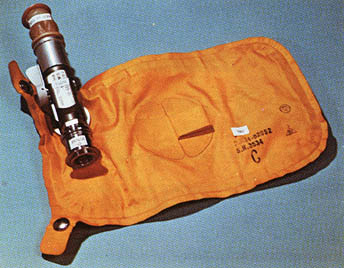
\includegraphics[width = 0.6\linewidth]{figs/apollo_urine_bag.jpg}
        \caption[Apollo Urine Transfer System]{Apollo urine transfer system.}
        \label{fig:apollo_urine_bag}
    \end{figure}

    Above in Figure \ref{fig:apollo_urine_bag} in which it had two main purposes: 1) dumping during time of voiding, and 2) dumping subsequent to voiding. This was a simple design but was only suitable for those with male appendices, thus this method is not suitable for the Lunar Loo Challenge.

    \begin{figure}[h]
        \centering
        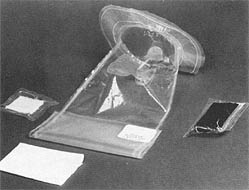
\includegraphics[width = 0.6\linewidth]{figs/apollo_fecal_bag.jpg}
        \caption[Apollo Fecal Bag]{Apollo fecal bag for defecating in microgravity.}
        \label{fig:apollo_fecal_bag}
    \end{figure}

    As shown above in Figure \ref{fig:apollo_fecal_bag}, the bag used to collect astronaut defecation's was rudimentary in design resulting in many of the astronauts being in great discomfort when defecating. This bag was placed over the anus of the astronaut, and would be sealed after use to prevent the spread of bacteria and pathogens. Again, like before this is not a suitable design for the Lunar Loo Challenge as this design is not reusable and may result in unwanted transfer of pathogens.
    


    \pagebreak
    \subsection{NASA's Skylab Waste Collection System}
    After the Apollo Era, attention in space was shifted to more long duration missions. These missions where based on Skylab, essentially the first manned space station in which many microgravity experiments took place and studies were conducted on the effects on the human body.

    \begin{figure}[h]
        \centering
        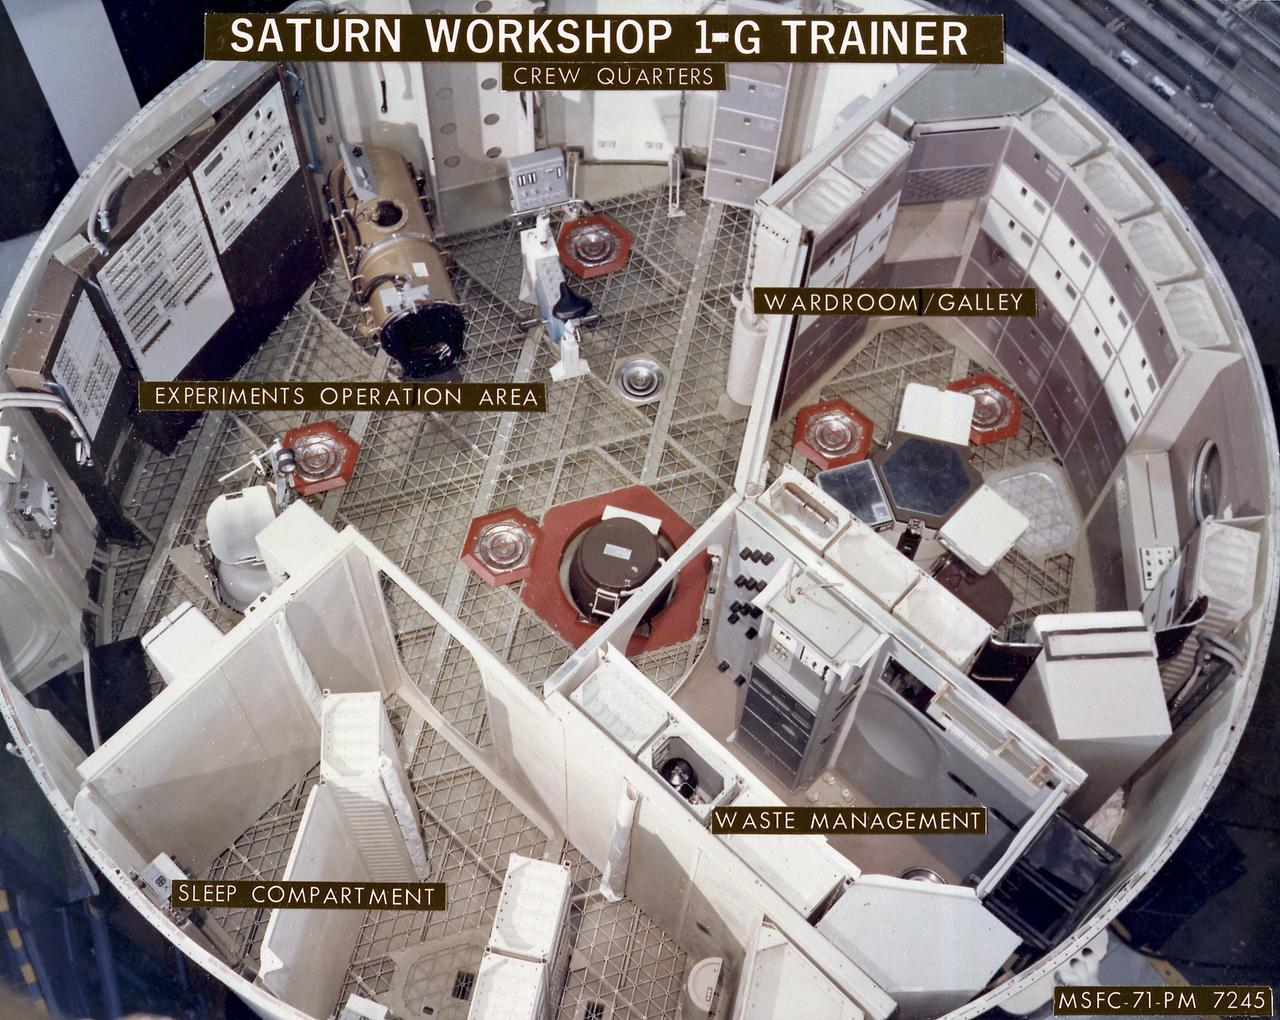
\includegraphics[width = \linewidth]{figs/skylab_overview.jpg}
        \caption[NASA's Skylab Crew Quarters]{Overview of NASA's Skylab trainer crew quarters.}
        \label{fig:skylab_overview}
    \end{figure}

    Above in Figure \ref{fig:skylab_overview} is the layout of Skylab workshop 1-G trainer crew quarters. The section labeled ``WASTE MANAGEMENT'' was the first implementation of a space waste management system instead of the more ``manual'' methods first demonstrated during Apollo.

    Essentially the space toilet was a small hole in the wall with a fan to direct airflow to pull in any urine and fecal matter. After defecating, Skylab would vacuum-dry their feces with heat to kill any pathogens and then be dumped into a waste tank or be studied for scientific purposes.\cite{ref:skylab_ref}

    \pagebreak
    \subsection{Space Shuttle's Waste Collection System}
    The toilet on the space shuttle was the first implementation of a space toilet and as such it was not easy to use. The opening was less than 4 inches wide, which is significantly smaller than a toilet on Earth. 

    \begin{figure}[h]
        \centering
        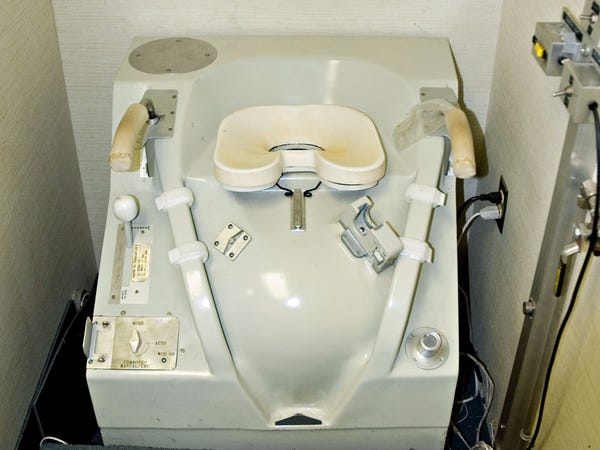
\includegraphics[width = \linewidth]{figs/space_shuttle_toilet.jpeg}
        \caption[Space Shuttle's Waste Collection System]{Space Shuttle's waste collection system.}
        \label{fig:sapce_shuttle_toilet}
    \end{figure}

    As shown above in Figure \ref{fig:sapce_shuttle_toilet}, this design was inspired by western style toilets but had its appropriate variations. This toilet was outfitted with fasteners to hold down the astronauts to prevent them from floating off while using the toilet. Then a vacuum-cleaner-like machine (not pictured) would suck up the wastes from the astronauts where the waste would later be vacuum dried before storing.

    Again, this was the first implementation of a space toilet, so there remained several key issues that needed improving such as.\cite{ref:space_shuttle}

    \begin{enumerate}
        \item No paper was allowed in the toilet, and had to be thrown out separately
        \item Astronauts had to be ``toilet trained'' on Earth, this training device included a camera to perfect their aim
    \end{enumerate}


    \pagebreak
    \subsection{Soyuz Waste Collection System}
    The Soyuz waste collection system is fairly simple in design taking a rather small form factor while remaining relatively functional. This design implements a vacuum suction to gently pull urine or fecal matter to the waiting filters to the storage containers.

    \begin{figure}[h]
        \centering
        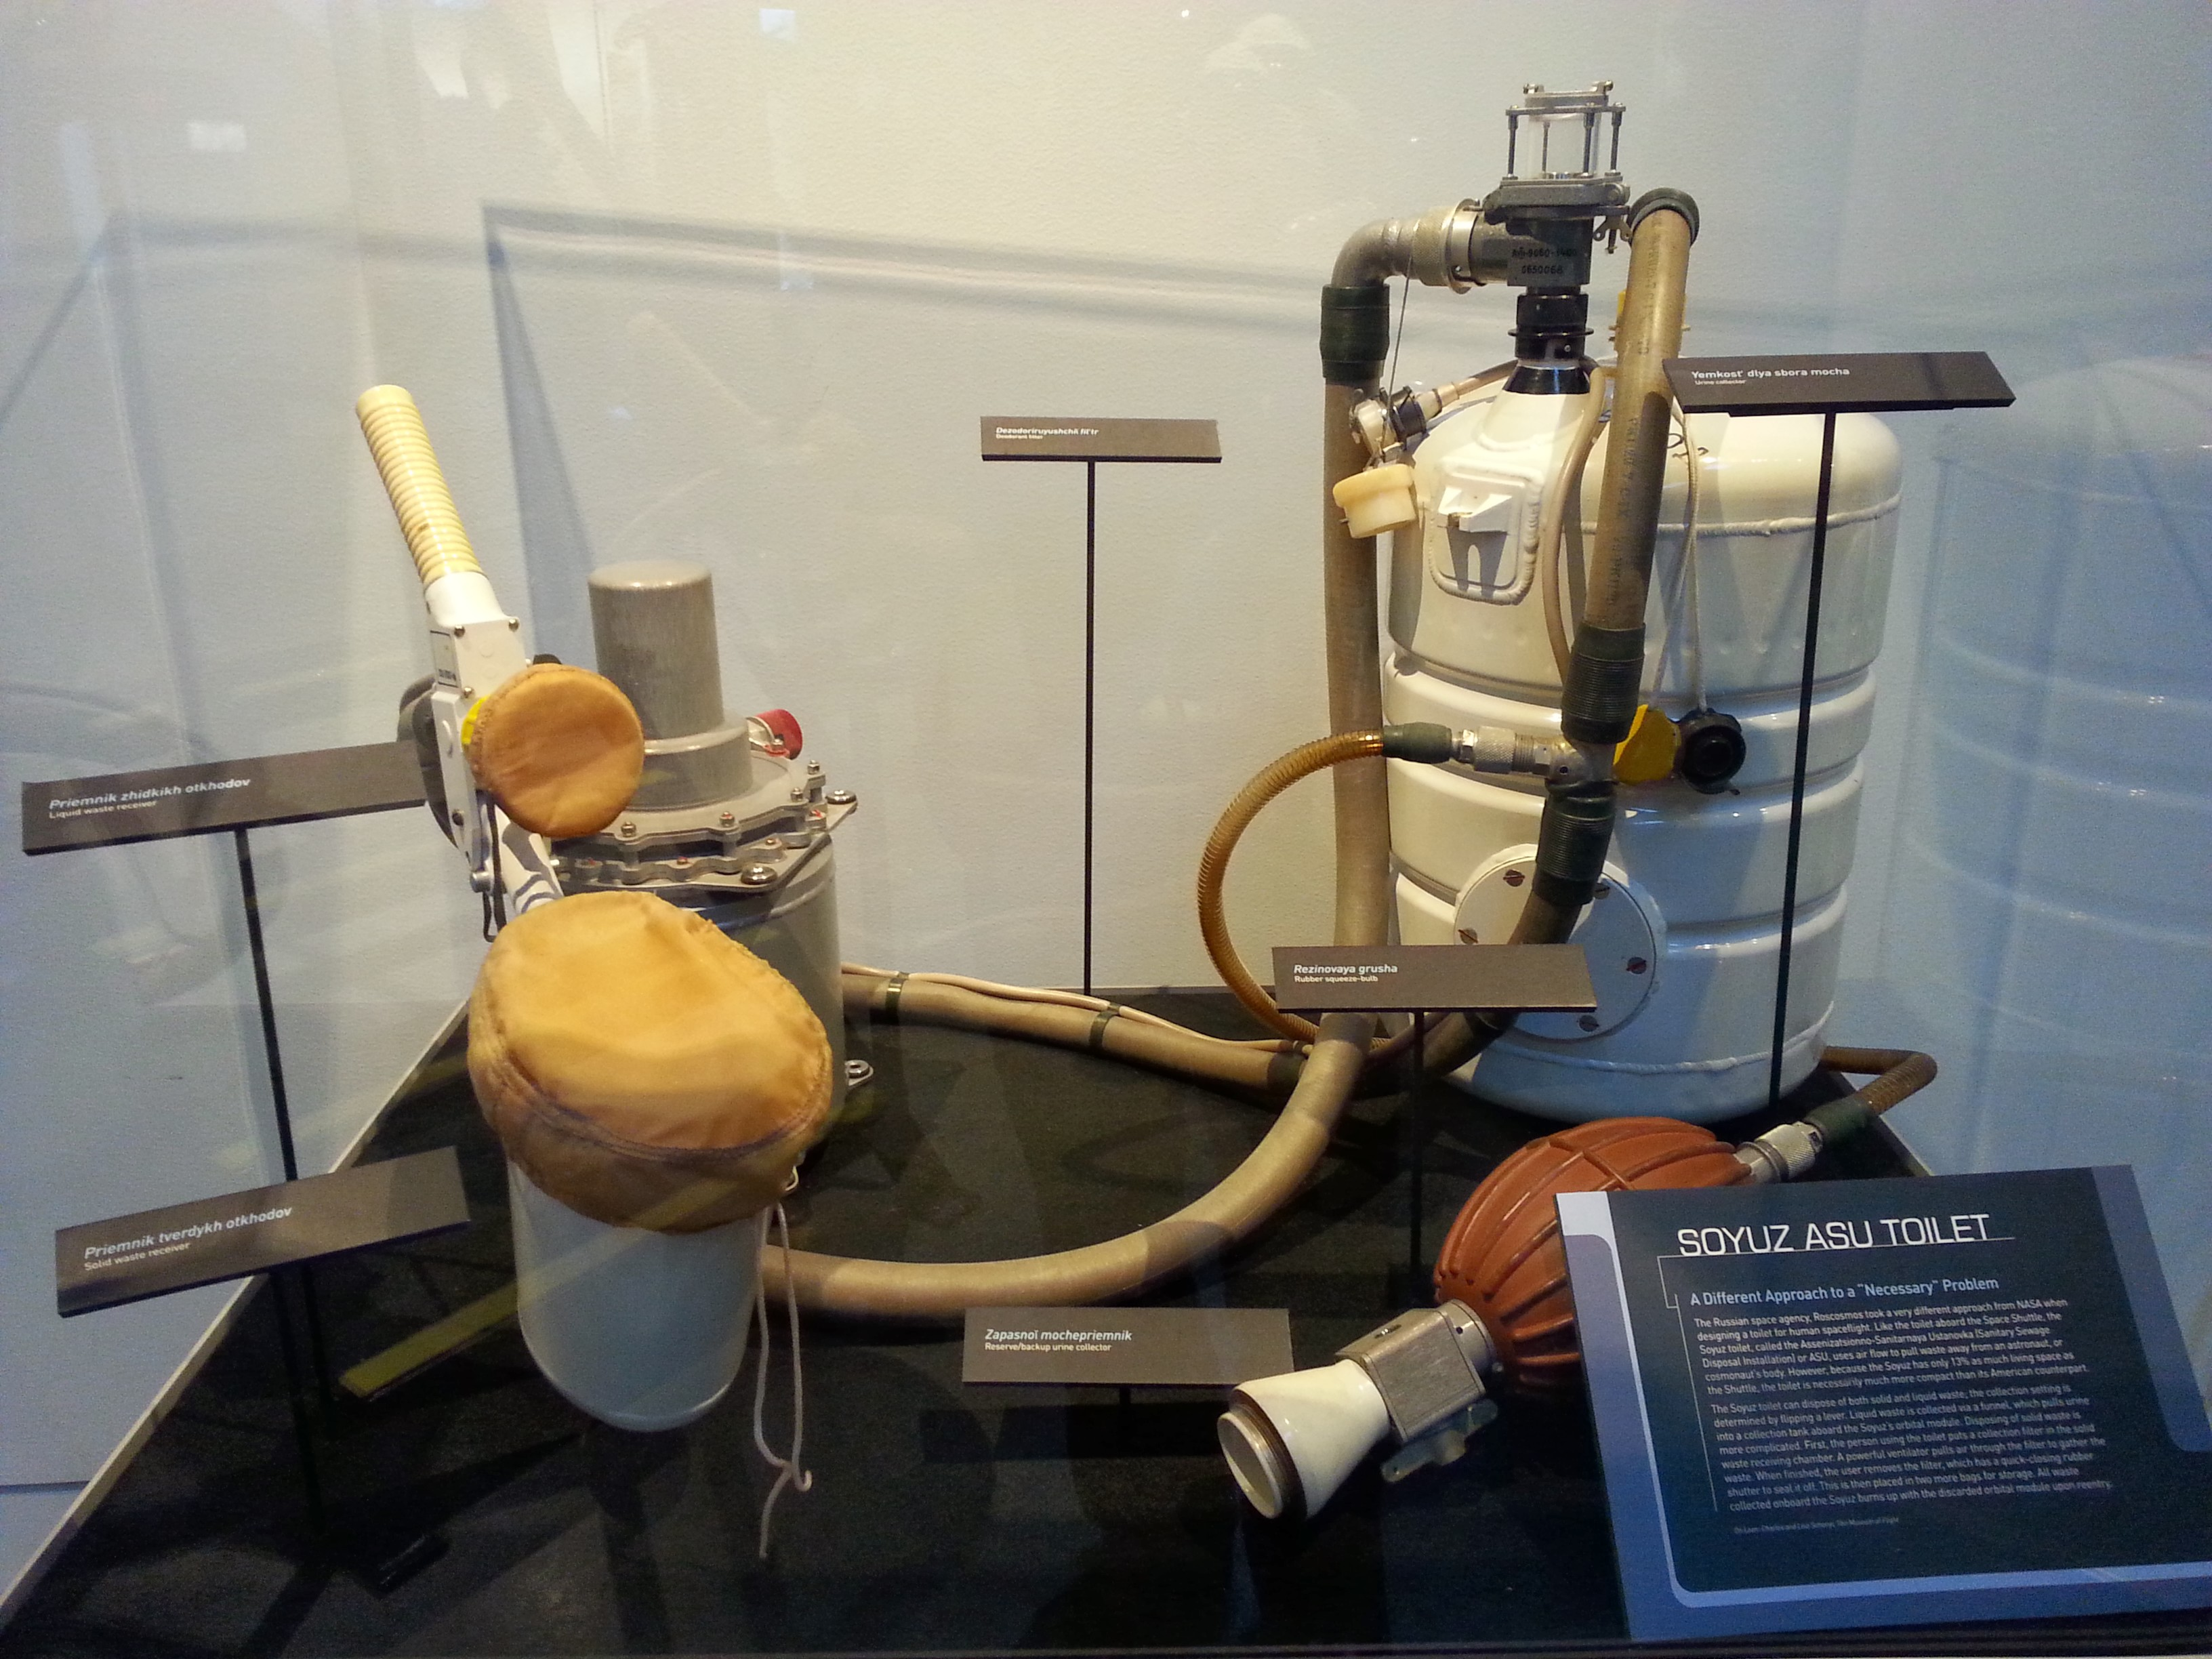
\includegraphics[width = \linewidth]{figs/soyuz_space_toilet.jpg}
        \caption[Soyuz Waste Collection System]{Soyuz waste collection system.}
        \label{fig:soyuz_space_toilet}
    \end{figure}

    Shown above in Figure \ref{fig:soyuz_space_toilet}, is the Soyuz implementation of a waste collection system that is extremely space efficient. This simple system has a small funnel that can aid in defecating and a small ``urinal'' for when urinating. However, as with all the other designs this design falls short when considering the compatibility between men and women.\cite{ref:soyuz_toilet}

    \pagebreak
    \subsection{International Space Station Waste Collection System}

    \begin{wrapfigure}[21]{l}{0.5\textwidth}
        \vspace{-1em}
        \centering
        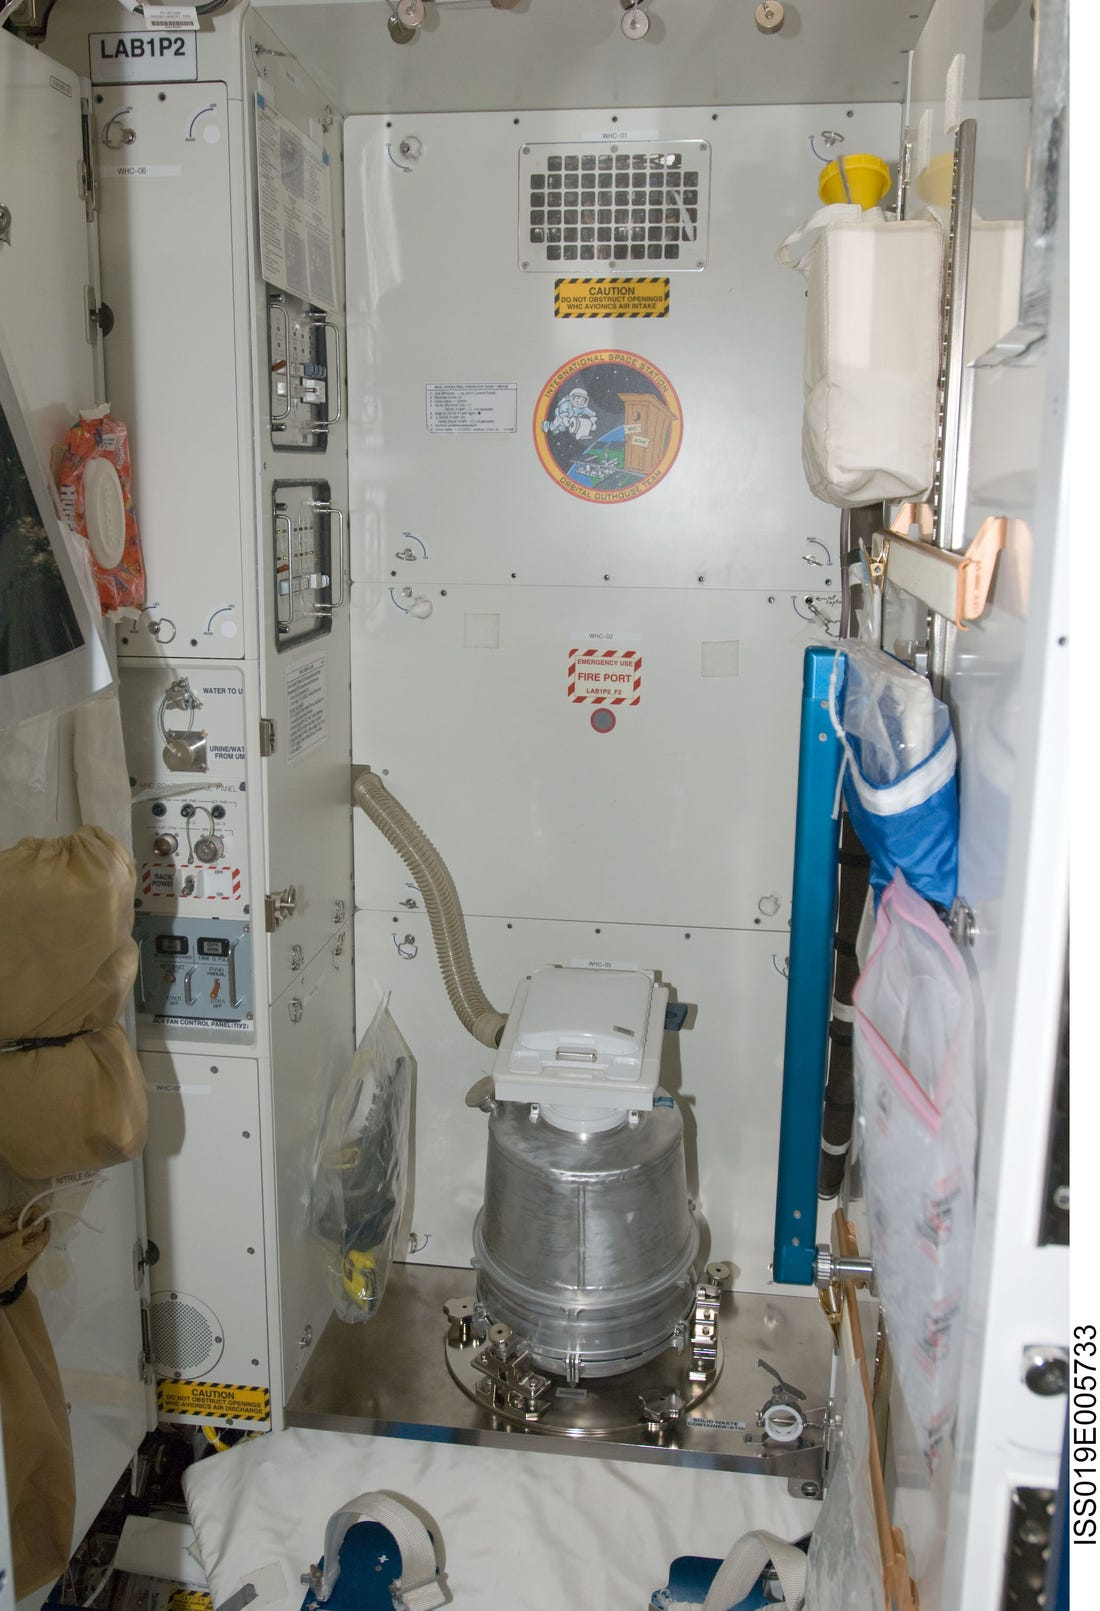
\includegraphics[width = \linewidth]{figs/iss_space_toilet.jpeg}
        \caption[ISS Waste Collection System]{ISS waste management and water recovery system.}
        \label{fig:iss_space_toilet}
    \end{wrapfigure}

    More advancements were made from the space shuttle and this resulted in the waste and hygiene compartment. This system would allow the unit to separately channel liquids and solid waste and store each separately. The solid waste would go to a holding tank whereas the urine would go to a recycling program to turn the crew members' urine into drinkable water. \cite{ref:iss_background}

    As shown to the left in Figure \ref{fig:iss_space_toilet}, the toilet had simplified in design and was interfaced with a water recovery system to allow for reclamation of waste water. This is an essential service for space travel since water is dense such that transporting it to space is costly and cost-analysis shows that reclamation is more cost effective long term. 

    Again, like the other waste collection systems, this system is based around vacuum suction to direct the waste to storage. However, where this design falls short is that it has separate attachments for men and women when absorbing urine. \cite{ref:iss_bathrrom} In this case the Lunar Loo Challenge would like one design that accommodates both men and women without the need of external attachments.
 
    \pagebreak
    \begin{minipage}[t][0cm]{\linewidth}
        {\Huge \textbf{References}}
        {\vspace{0.5cm}\vskip-\ht\strutbox\makebox[\textwidth][c]{\rule{\dimexpr\textwidth}{2pt}}\par}
        \addcontentsline{toc}{section}{References}
    \end{minipage}
    
    {\printbibliography[heading=none]

    \thispagestyle{empty}}


